\documentclass{cwru}

\title{Exploring Alternative Routes Using Multipath TCP}
\author{Stephen Brennan}
\date{June, 2017} % Graduate date
\doctype{thesis}
\degree{Master of Computing and Information Science}
\department{Electrical Engineering and Computer Science}

\defensedate{June 2, 2017}

\usepackage{listings}
\usepackage{graphicx}
\usepackage{color}
\usepackage{fancyvrb}
\usepackage{acro}
\definecolor{mygreen}{rgb}{0,0.6,0}
\definecolor{mygray}{rgb}{0.5,0.5,0.5}
\definecolor{mymauve}{rgb}{0.58,0,0.82}
\lstset{%
  backgroundcolor=\color{white},     % background color
  basicstyle=\footnotesize\ttfamily, % monospace, small font
  breaklines=true,                   % nice line breaks
  captionpos=b,                      % put captions at bottom
  commentstyle=\color{mygreen},      % comments
  escapeinside={(*}{*)},             % if you want to add LaTeX in code
  keywordstyle=\color{blue},         % keyword
  stringstyle=\color{mymauve},       % string
}

\DeclareAcronym{mptcp}{
  short = MPTCP,
  long  = Multipath TCP
}
\DeclareAcronym{dss}{
  short = DSS,
  long  = Data Sequence Signal
}

\begin{document}
\advisor{Michael Rabinovich}
\committee{Vincenzo Liberatore}
\committee{Mark Allman}

% The organization of the dissertation must follow the order below:
%
% Title page
% Committee Approval Sheet
% Copyright page (only if copyrighting)
% Dedication page (optional)
% Table of Contents
% List of Tables
% List of Figures
% Preface (optional)
% Acknowledgements (optional)
% List of Abbreviations (optional)
% Glossary (optional)
% Abstract
% --TEXT--
% Appendix
% Bibliography

\maketitle
\makeapprovalsheet

\frontmatter
\tableofcontents

\cleardoublepage
\phantomsection
\addcontentsline{toc}{chapter}{List of Figures}
\listoffigures

%\begin{acknowledgments}
%\lipsum[1-3]
%\end{acknowledgments}

% If you're using `glossaries` package

%\cleardoublepage
%\phantomsection
%\addcontentsline{toc}{chapter}{List of Acronyms}
%\printglossary[type=\acronymtype]

%\cleardoublepage
%\phantomsection
%\addcontentsline{toc}{chapter}{Glossary}
%\printglossary

% because they were probably used above
\acresetall

\begin{abstract}
Abstract abstract abstract.
\end{abstract}

\mainmatter
\chapter{Introduction}

In recent years, several forces have driven the development of the Internet.
Residential bandwidth has increased, and residential fiber connections are
becoming more common. % citation needed?
While conventional wisdom has been that access links are usually the bottleneck,
this is not always the case \cite{akella2003empirical}. While they have
increased, studies have shown that residential link bandwidths are not fully
utilized, especially fiber connections \cite{fibertothehome}. While there are
many explanations for this, one possibility is that bottlenecks have moved to
within the network core.

It is sometimes the case that paths other than the Internet routed one show
superior connection properties between two hosts. This could be due to poor
routing metrics, restrictive routing policies, or manual traffic shaping on the
part of Internet service providers \cite{detour}. Savage \textit{et al.} have
shown that by adding a ``detour'' host into a path, latency and packet drop
rates can be reduced.

Overlay routing systems have been developed as a way to leverage this, as well
as to provide services not widely available on the general Internet, such as
multicasting \cite{ron,mbone,jannotti2000overcast}. While overlay networks are
able to provide new and interesting features, they are typically limited by
deployment or implementation details.

In parallel to the development of these overlay systems, another set of changes
began to emerge. Devices with multiple interfaces started to become common, both
in consumer devices and data center devices. The \ac{mptcp} extension was
developed to allow TCP connections to take advantage of multiple network
interfaces, and thus multiple routing paths. It provides a TCP-compatible
service to applications, allowing pre-existing applications to use \ac{mptcp},
simply by upgrading the operating system.

However, \ac{mptcp} is not limited just to devices with multiple network
interfaces. A \ac{mptcp} connection consists of multiple TCP subflows, and the
specification is general enough to allow these subflows to belong to the same
network interfaces, but traverse a different path. As a result, \ac{mptcp} could
be used to route connections across a detour. In this thesis, we implement and
evaluate a mechanism for doing just that. Our system is based on version 0.91 of
the \ac{mptcp} implementation for the Linux kernel \cite{mptcp}. We find that
this system is capable of aggregating the throughput multiple paths, without any
additional network interfaces.

\section{Multipath TCP}
% Our discussion of Multipath TCP needs to be in enough depth that the reader
% understands how it works - essentially covering at least the first few pages
% of the RFC. In particular:
% - Subflows: what they are and how they work
% - How the initial subflow is created
% - How subsequent subflows are created and authenticated
% - Data sequencing and how data sequences are mapped onto subflow sequences
% - path management and data scheduling
% - ? how the linux kernel implementation is structured

Recently, multi-homed devices have become increasingly common. The most obvious
example of these devices is the smartphone, which typically comes with at least
two network interfaces: one for cellular data, and one for Wi-Fi. While these
devices have become more common, most Internet protocols do not have ways to
take advantage of multiple interfaces.

\ac{mptcp} is an extension to TCP which aims to mitigate this problem. It is
designed with the following goals in mind \cite{rfc6824}.

\begin{itemize}
  \item To improve both the throughput and reliability of connections, relative
    to normal TCP.
  \item To remain compatible with applications that use TCP, so that they could
    use \ac{mptcp} without modification.
  \item To remain compatible with the Internet as a whole, especially with
    ``middleware'' such as firewalls, proxies, and NATs.
\end{itemize}
% https://tools.ietf.org/html/rfc6182#section-2

\begin{figure}[h]
  \centering
\begin{BVerbatim}
                             +-------------------------------+
                             |           Application         |
+---------------+            +-------------------------------+
|  Application  |            |             MPTCP             |
+---------------+            + - - - - - - - + - - - - - - - +
|      TCP      |            | Subflow (TCP) | Subflow (TCP) |
+---------------+            +-------------------------------+
|      IP       |            |       IP      |      IP       |
+---------------+            +-------------------------------+
\end{BVerbatim}
\caption[Comparison of TCP and \acs{mptcp} Protocol Stacks]{Comparison of
  Standard TCP and \ac{mptcp} Protocol Stacks. Originally from \cite{rfc6824}}
  \label{fig:layers}
\end{figure}

To achieve these goals, \ac{mptcp} is located between TCP and the application
layer, as shown in Figure~\ref{fig:layers}. To applications which aren't aware
of \ac{mptcp}, the interface is exactly the same as TCP, accessed through the
same socket operations and interface.

A \ac{mptcp} connection begins similarly to a TCP connection, but with the
addition of the TCP option with subtype \texttt{MP\_CAPABLE}. Additional TCP
connections (referred to as ``subflows'') may be created between the two hosts
once the initial one is established, using the \ac{mptcp} option subtype
\texttt{MP\_JOIN}.

Data has sequence numbers at both the subflow level and at the connection level.
Each subflow has a \ac{dss} negotiated via the \ac{mptcp} option subtype
\texttt{DSS}, which maps subflow sequence numbers to data sequence numbers. Data
is acknowledged both at the subflow level (via the \texttt{SYN} flag), and at
the data level (via a flag within the \ac{dss}).

As a result of this flexibility in labeling data with sequence numbers, data may
be split up across multiple subflows, or even transmitted redundantly. In the
Linux kernel implementation, determining how data should be split up is the job
of a modular component called a scheduler \cite{mptcp}. The default scheduler
implementation selects the subflow with the smallest RTT and fills up its
congestion window. Other implementations include a naive round-robin scheduler
and one which sends data redundantly across each subflow. Additional schedulers
have been proposed, to mitigate problems such as head-of-line blocking and
bufferbloat \cite{paasch2014experimental}. In this thesis, we consider only the
Lowest-RTT First scheduler.

An implementation may establish a new subflow with its peer at any time, using
the same address, or using a new one. Additional addresses may be passively
advertised using the \ac{mptcp} option subtype \texttt{ADD\_ADDR}, and they may
be removed via the \ac{mptcp} option subtype \texttt{REMOVE\_ADDR}. These
options are not reliably transmitted, so they are purely informational. While
either side of a connection may initiate a new subflow, it is expected that the
client initiate most subflows.

In order to decide when to create and destroy new subflows, the Linux
implementation uses another modular component called a ``path manager''
\cite{mptcp}. The default implementation does nothing (except accepting incoming
connections). The Linux implementation also includes an \texttt{ndiffports} path
manager, which initiates up to $N$ subflows with a server, from different source
ports. A \texttt{fullmesh} path manager establishes subflows between every pair
of client addresses and advertised server addresses. A major part of the
implementation of this thesis is a path manager for the Linux kernel \ac{mptcp}
implementation.

\section{Netfilter}
% Discuss what it is, and how it can be used to perform NAT

\section{OpenVPN}
% This will have to at least touch on TUN/TAP devices, and the variations of the
% OpenVPN protocol.


\chapter{Related Work}
% Binder
% SCTP
\section{Detour Routing}
% this feels more like background than related work... this motivates the whole
% project really.


\chapter{Implementation}
% Section intro:
% 1. Expectations (what hosts are there, and which ones run our code?)
% 2. Overview of the distinct pieces of software (client kernel, client daemon,
%    detour daemon)
% Subsection - Detour daemon
% Subsection - Client kernel
% Subsection - Client daemon

% smoother transition once we have everything

In this project, we implement a system which allows one host to dynamically add
new overlay routes to a Multipath TCP connection. Each overlay route is a new
subflow, which is tunneled across a third-party host. The system involves at
least three hosts:
\begin{itemize}
\item The \emph{client} is the host which adds detour routes, attempting to
  improve its connection quality. The client must be the host which initiates
  the \ac{mptcp} connection.
\item The \emph{server} is the host with which the client wishes to communicate.
\item The \emph{detour} is a host which acts as a waypoint along the overlay
  route from the client to the server. It tunnels the \ac{mptcp} between them. There
  may be more than one detour at a time.
\end{itemize}

We assume only that the server supports Multipath TCP, and require no additional
customization for our system to work. In our current implementation, the detour
host must run some version of Linux, and the client must run a custom version of
Linux.

The system is implemented via a number of interacting components. First, a path
manager extension for version 0.91 of the Linux \ac{mptcp} implementation
\cite{mptcp}, which allows the client's kernel to request new detour paths,
receive them, and create subflows across them. Second, a user-space utility
which receives messages from the kernel and creates the necessary detour paths.
Finally, we implement two different types of detour daemons, which run on the
detour host. These components are illustrated in Figure~\ref{f:MovingParts}.

\begin{figure}[h]
  \centering
  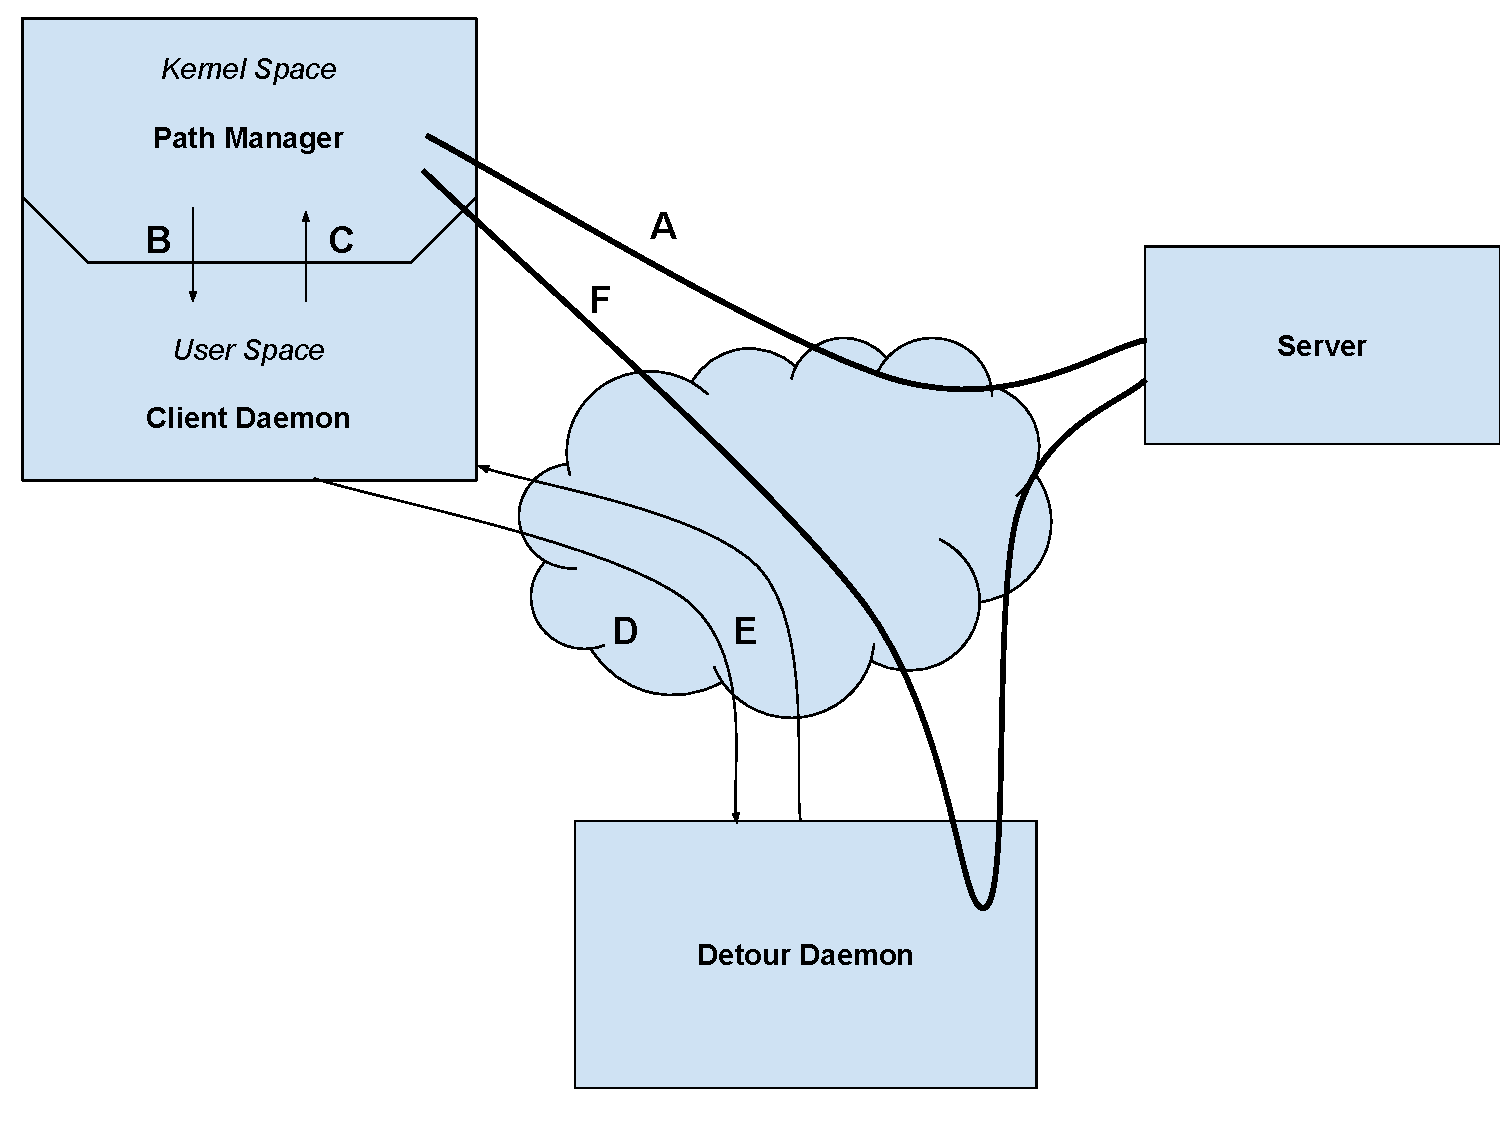
\includegraphics[width=\textwidth]{figures/MovingParts.pdf}
  \caption[Interaction of client, detour, and server]{
    The components and their communications. In \textbf{A}, the path manager
    requests an overlay route. In \textbf{B}, the client daemon reports overlay
    routes back to the path managers. In \textbf{C} and \textbf{D}, the client
    and detour daemons negotiate an overlay route. In \textbf{E}, a subflow is
    created through the detour.
  }
  \label{f:MovingParts}
\end{figure}

The typical interaction of these components is as follows. First, the client
creates a \ac{mptcp} connection to the server. The first subflow uses the Internet
routed path. Once this connection is fully established, the path manager
requests overlay routes on which it may create subflows. The client and detour
daemons negotiate a tunnel, which may be implemented in two different ways. The
client reports this to the path-managers, which creates subflows for the \ac{mptcp}
connection across every available detour, until a predefined limit is reached.

In the remainder of this section, we will discuss each of these components at
length.

\section{Detour Daemon}

We have implemented two different mechanisms for tunneling \ac{mptcp} subflows across
a detour. In both cases, the detour host must run a daemon that assists in
tunneling traffic from the client to the server.

\subsection{OpenVPN Tunneling}

The first mechanism involves the open-source tool OpenVPN. Detours run a
specially configured OpenVPN server. Clients connect to this VPN, creating a
virtual network device. The client receives a routing rule from the detour
advertising that it can reach all hosts on the Internet with a very high cost.
As a result, the client operating system will prefer other routes to the VPN.

The VPN connection is configured as follows:

\begin{itemize}
\item The connection is over UDP, to avoid the so-called ``TCP Meltdown'' effect
  caused by two congestion control algorithms interfering with each other.
  % TODO citation
\item The initial connection negotiation requires the client and server to
  exchange certificates.
\item Subsequent messages are not protected by encryption or signatures, to
  avoid overhead.
\end{itemize}

One important aspect of VPN configuration is that the detour must create a
private IP subnet. It will provide a DHCP service in order to assign IP
addresses to clients as they connect to the VPN. Clients are expected to be able
to connect to multiple detours simultaneously. In order to do this without
conflict, each detour must use a distinct private IP subnet, so that there is no
chance of the client addresses overlapping, and also so that the gateway address
of the VPN is unique on the client.

In a large-scale implementation of this technology, these subnet allocations
could be handled by a centralized detour management server. The 10.0.0.0/8
subnet is reserved for private networks, and if each detour were to establish
its own /24 subnet, there would be capacity for 65,536 non-conflicting subnets.
However, in our testing, subnets were manually allocated to avoid conflicts.

Finally, in order to forward VPN traffic to the internet, the detour must be
configured (via Netfilter) to perform network address translation (NAT) on
outgoing packets. This process is typical for a home router and for VPNs which
provide Internet access. Multipath TCP is designed with this behavior in mind,
and so it is capable of functioning through NAT, so long as the middleboxes do
not remove TCP options in transit.

% TODO cite MPTCP design/architecture for middleboxes

The OpenVPN implementation has several attractive qualities. First, it relies on
a well-used protocol for forwarding traffic. Second, it need not be configured
on a per-connection basis. Finally, it provides a built in mechanism for
mutually authenticating the client and detour. However, there are some
drawbacks. Since packets are tunneled, at least 28 bytes of overhead (IP and UDP
headers) are required. To avoid fragmentation, the connection's maximum segment
size (MSS) may need to be adjusted, although in our testing, this was not
required.

\subsection{NAT Tunneling}

The second approach directly modifies packets, without actually using a protocol
(like OpenVPN) for tunneling. Since we only need to forward some connections to
some destinations, the full power of OpenVPN is not necessary. Instead, packets
are addressed directly to the detour. The detour can forward these to the
final destination, and forward reply packets to the client. In order to do this,
the detour must have advance knowledge of the final destination of the packet.
So, clients use a simple signaling protocol to request tunnels via a detour.

The Linux kernel's Netfilter framework allows for two types of NAT. The first
kind, source NAT (SNAT), rewrites the source address of the packet. This is
the typical form of NAT used by home routers: the source address of an outgoing
connection is rewritten to be the router's external IP address, but the
destination is unchanged. The second kind of NAT supported by Netfilter is
destination NAT, or DNAT. This rewrites the destination address of the packet.

% TODO - netfilter docs citation

The detour takes advantage of both forms of NAT offered by the kernel. First, it
applies DNAT, setting the destination address to be the final server's IP
address (arranged ahead of time). Then, it applies SNAT, setting the source
address to be its own external IP. The Netfilter framework remembers these
connections so that reply packets are properly forwarded back to the client.

Thanks to Netfilter, this NAT mapping can be arranged with two \texttt{iptables}
commands, with no custom kernel or user-space code required for packet
forwarding. It is possible to implement this in userspace using raw sockets, but
this approach has several drawbacks. It would have to be single-threaded, and it
would require that packet data be copied from kernel space into user space and
back. More critically, the connection tracking provided by the kernel is more
robust than what would be implemented by user space.

As mentioned earlier, the server address must be communicated to the detour
ahead of time in order to use this scheme. To that end, we have designed a
simple UDP-based for clients to ``request'' NAT mappings from a detour. The
detour listens for requests on UDP port 45672. The request format is shown
in Figure~\ref{fig:udp-nat-packet}.

\begin{figure}
  \centering
\begin{BVerbatim}
+-----------------------------------+
| ver(1) | op(1)  | reserved (2)    |
+-----------------------------------+
|           rip (4 bytes)           |
+-----------------------------------+
| rpt (2 bytes)   | dpt (2 bytes)   |
+-----------------|-----------------+
\end{BVerbatim}
  \caption{UDP NAT tunnel request structure}
  \label{fig:udp-nat-packet}
\end{figure}

The \texttt{ver} field is a protocol version, currently set to 1. The
\texttt{op} field contains the operation of this message: request (0) or
response (1). The \texttt{reserved} field is unused, currently existing to pad
the request. The field \texttt{rip} (short for ``remote IP'') is the address
that the client wishes to create a detour to. \texttt{rpt} is the TCP port on
the server to create a detour to. To understand the \texttt{dpt} field, it is
useful to describe all of the addresses and ports in use during a tunneled
connection:
\begin{itemize}
\item Client IP, port: the IP address of the client, and the client-side port,
  which is usually ephemeral.
\item Detour IP, port (client side): the IP and port that the client will
  address its communication to.
\item Detour IP, port (remote side): the IP and port which are used when the
  detour opens its corresponding connection on the remote.
\item Remote IP, port: the IP and port which the client is tunneling its
  connection to.
\end{itemize}

The \texttt{dpt} field corresponds to the detour port, client side. In a
request, the client proposes a port. In the response, the detour specifies the
actual port which will be used. The server may wish to alter the \texttt{dpt}
field for several reasons:
\begin{itemize}
\item A tunnel to the remote IP, port pair is already open on a different detour
  port.
\item The client already has a detour open (to a different remote) on the given
  port.
\item The detour may have a socket accepting connection on the proposed port,
  and so it may wish to avoid creating a tunnel which would prevent the client
  from accessing that service.
\end{itemize}

In order to create the tunnels, the detour runs two IPTables commands, which
create NAT rules. The first performs DNAT:

\begin{lstlisting}
iptables -t nat -A PREROUTING \
         -s (*\emph{ClientAddress}*) \
         -d (*\emph{DetourAddress}*) \
         -p tcp --dport (*\emph{DetourPort}*) \
         -j DNAT --to (*\emph{RemoteAddress}*):(*\emph{RemotePort}*)
\end{lstlisting}

In this command, we add to the \texttt{nat} table, on the \texttt{PREROUTING}
chain. Incoming packets from the client, addressed to the agreed upon
\textit{DetourPort} are sent to the \texttt{DNAT} chain, which rewrites the
destination address to be the agreed upon remote address and port. This must
occur before the kernel routes the packet. Once the kernel has routed the
packet, the DNAT rule can be applied:

\begin{lstlisting}
iptables -t nat -A POSTROUTING \
         -s (*\emph{ClientAddress}*) \
         -d (*\emph{RemoteAddress}*) \
         -p tcp --dport (*\emph{RemotePort}*) \
         -j SNAT --to (*\emph{DetourAddress})
\end{lstlisting}

Since the destination address and port have already been modified, this rule
looks for packets addressed to the remote address and port, but still using the
client address as the source. It jumps these packets to the DNAT chain, where
their source address will be rewritten as the detour's address.

It is important to understand that these rules are generally only applied to the
initial SYN segment of the TCP flows. Once these rules are applied, the
connection tracking mechanism of the kernel takes over, ensuring that these
rules are applied in reverse to response packets.

The detour daemon is implemented as a Python script. It listens for tunnel
requests, executes the correct commands to create them, and then sends
responses. It ensures that detour ports do not collide with each other, or with
ports that are open on the daemon machine. It also ensures that on termination,
all tunnels are torn down.

This mechanism has the advantage that it requires zero overhead. Since no
headers are added, the full amount of data may be transmitted on these segments.
However, its disadvantage is that tunnels must be configured each time a new
connection is created on the client. While the client may simply send packets to
a new remote through an OpenVPN tunnel, it must incur a RTT delay requesting a
new tunnel from the NAT detour before it can begin establishing a subflow.

\section{Path Manager}

To enable subflows to use the detours created above, we implement a custom \ac{mptcp}
path manager within the Linux kernel. The path manager is a module which
dictates local policy for creating new subflows and announcing local addresses.
For example, the \texttt{fullmesh} path manager creates a subflow between each
address on the client and server.

The path manager receives space within the \ac{mptcp} control buffer in order to
track state, and it registers a set of callbacks with the protocol, so that it
can be notified of events as they occur. Our path manager (named
\texttt{detour}) runs a worker when a client-side \ac{mptcp} connection becomes fully
established (i.e. after the three-way handshake completes). The first thing this
is send a message to userspace, requesting a detour. Then, it looks through an
internal list of detours. The kernel maintains two lists of detours (per network
namespace). The first is a list of OpenVPN detours. These detour entries are not
specific to a server, and they simply indicate the name of a network interface
to use. The second list contains NAT detours. These consist of a detour address
and port, and a server address and port. The worker may only select NAT entries
which match the server address and port of the connection it is working on.

The task attempts to add up to $N$ subflows, where $N$ is a configurable limit.
It terminates in one of two ways. Either it has exhaused all of the available
detours, but not yet created all $N$ subflows. Otherwise, if it creates $N$
subflows successfully, it stops looking through the list, even if more detours
are available. If OpenVPN detours are available, then they take precedence over
the NAT detours, because they are available immediately. NAT detours created by
the client daemon become available only once the daemon has processed the
request from the kernel.

The kernel listens for new detour routes. When it receives them, it adds them to
the appropriate internal list. Then, it iterates over every \ac{mptcp} connection
within the network namespace of the message, waking their workers to give them
the opportunity to create a new subflow along this detour. If the detour was
OpenVPN type, every worker notified. If the detour was NAT type, then only
connections which match the server address and port are notified.

\section{Client Daemon}

The client daemon has several responsibilities. First, it must create OpenVPN
connections report them to the kernel. Second, it must respond to detour
requests from the kernel by creating NAT detours and reporting them back.

The daemon has a configuration file which allows the user to specify the IP
addresses of hosts to use for both types of detours. On startup, the daemon
connects to each OpenVPN detour and reports the resulting network interfaces to
the kernel. Then, it waits listening for detour requests from the kernel. For
each request, it requests a detour from every NAT detour address. Upon receiving
responses, it sends them the the kernel as well.

\subsection{Client Communication}

In order to communicate between kernel and userspace, we use Generic Netlink
sockets. Netlink is an address family for the socket interface
(\texttt{AF\_NETLINK}, similar to \texttt{AF\_INET}), which allows communication
between kernel and userspace. Many existing Linux network configuration
utilities communicate with the kernel over the Netlink address family, such as
route and firewall configuration. Each of the subsystems being configured has a
corresponding protocol family, such as \texttt{NETLINK\_NETFILTER} for Netfilter
firewall configuration. These protocol families take the same place in the
\texttt{socket()} system call as protocol families such as \texttt{IPPROTO\_TCP}
in the \texttt{AF\_INET} and \texttt{AF\_INET6} address families.

Creating a new Netlink protocol would involve allocating a new Netlink protocol
family. To make this process easier, the Generic Netlink protocol family was
created. It allows custom protocols (``Generic Netlink families'') to be
created, dynamically allocated, and discovered. It also provides a common format
for sending several data types, and creates a framework for defining message
types. Further, Generic Netlink provides a multicast capability, allowing kernel
and user sockets to broadcast messages to any socket which has joined a
particular multicast group. Finally, Generic Netlink comes with a kernel and
userspace library which allows for a consistent API and a level of abstraction
when defining Generic Netlink families.

To allow the kernel to request detours, and userspace to communicate the
existence of these detours, we define a Generic Netlink family. This protocol is
similar to the UDP protocol which the client daemon uses to request NAT tunnels.
The kernel sends a message of type \texttt{DETOUR\_C\_REQ} to a ``multicast
group'' which the client daemon subscribes to. This message contains the
parameters necessary for the daemon to create a tunnel: the server address and
port. The client daemon receives this message and creates tunnels, based on a
configuration file. It then reports these tunnels to the kernel, using a
\texttt{DETOUR\_C\_ADD} message type. The client daemon may also use the
\texttt{DETOUR\_C\_DEL} message type to delete a tunnel entry it has previously
added. Finally, the \texttt{DETOUR\_C\_ECHO} message type requests that the
kernel log all tunnels for diagnostics.

\backmatter
\appendix

\bibliographystyle{ieeetr}
\bibliography{paper}

\end{document}